\chapter{Introduction and Overview}

At first, let's review the goals of this course:\\
The main focus of this course is the science and technology of blockchain protocols and the applications built on top of them. Therefore, we will mainly discuss the fundamental principles of blockchain design and analysis.\\
 It’s worth recognizing that we’re currently in a particular moment
in time, witnessing a new area of computer science blossom before our eyes in real time. It draws on well-established parts of computer science (e.g., cryptography and distributed systems) and other fields (e.g., game theory and finance), but is developing into a fundamental and interdisciplinary area of science and engineering in its own right.

\section{Overview}
Here we start with the phrase "blockchain stack", in which stack refers to a bunch of layers each building on top of the previous one. To explain the organization of these lectures, it’s useful to keep in mind a cartoon version
of a “blockchain stack” that comprises a number of layers (Figure 1.1). Starting from the bottom and moving on up:\\
\begin{itemize}
    \item \textbf{Layer 0:} For us, layer 0 will basically be the Internet. That is, it provides at least a semi-reliable. Therefore, we are not assuming that the internet is perfect and we will be taking into account all the delays and possible attacks.
method for point-to-point communication between untrusted parties.
    \item \textbf{Layer 1:} Layer 1 is the consensus  layer, and its job is to keep a bunch of computers (potentially
    scattered all over the globe) in sync, despite possible network failures and attacks.
    For example, Bitcoin and Ethereum are both layer-1 protocols. For smart contract
    platforms like Ethereum, it can also be useful to separate out the compute layer, with
    the consensus layer merely deciding which instructions (smart contract function calls,
    etc.) should be executed and in what order, and the compute layer responsible for
    actually carrying out those instructions and updating the global state. (E.g., full
    nodes running the Ethereum protocol participate simultaneously in both consensus
    and compute. It means that because we're participating in a consensus protocol, you will be kind
    of working hard and talking to other
    full nodes so that you all stay in sync,
    but what it is you're staying in sync 
    on a platform like that is a sequence of
    instructions.So the consensus
    part is that you come to an agreement on the
    sequence of instructions that need to be
    carried out but then there's still the
    ta\textit{sk} of actually carrying out that
    computation. And again if you're running
    a full node in Ethereum, you're also
    responsible for the computation that
    you've come to consensus on.So that's a
    sort of concept of two conceptually
    distinct responsibilities and so
    sometimes it's worth a sort of formal
    differentiating between them)
    \item \textbf{Layer 2:} For us, layer 2 will be the scaling layer. The goal here is basically to implement the
    same functionality exported by a layer-1 protocol, but a lot more of it. So, layer two is really necessary when you're not happy
    with the sort of amount of processing
    power you have
    at your layer one.
    For example,
    Bitcoin and Ethereum can only process so many transactions (roughly 5 per second
    and 15-20 per second, respectively), and the point of a layer-2 protocol is to scale this capacity up by at least a couple of orders of magnitude.

    \item \textbf{Layer 3:} Finally, on top, there is an application layer (as there is in the Internet stack), which
    refers to the applications built on the functionality provided by the previous layers.
    (Decentralized exchanges like Uniswap and NFT marketplaces like OpenSea are examples you might be familiar with) Here again we’re grouping together two logically
    distinct things, the actual smart contracts that live in the blockchain (sometimes called the “protocol layer”) and the user-facing on top (e.g., a Web interface). For example, Uniswap consists of two things, its smart contracts and its Web interface to interact
    with those contracts. These are different things. For example, you can interact with the
    Uniswap contracts directly (as one would via a function call from a different contract,
    for example) rather than going through the standard Web interface.
\end{itemize}

Here is a cartoon version of the “blockchain stack” to explain the organization of this
lecture series:
\begin{figure}[h]
    \centering
    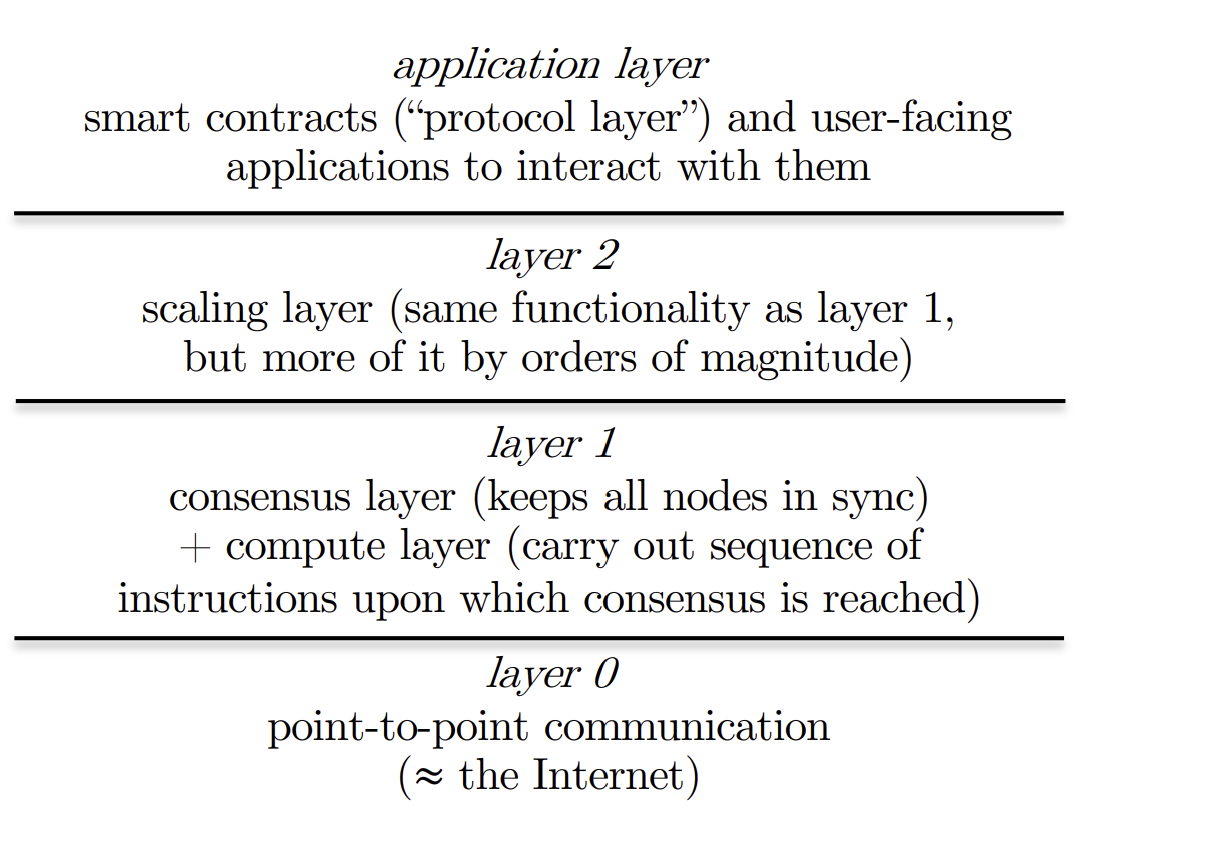
\includegraphics[scale = 0.7]{figures/f1.png}
    \caption{cartoon version of the “blockchain stack”}
    \label{fig:mesh1}
\end{figure}\\

Again, don’t take this taxonomy too seriously—it’s in flux and not at all standardized. For
example, “layer 2 solution” often means something more specific than an arbitrary scaling
solution (as we’ll discuss in a future lecture). Also, the clean picture of a stack is misleading,
as the boundaries between layers are porous. Ideally, the layers would be insulated from
each other, with protocols for one layer depending only on the provided functionality of
the layer below (and independent of the latter’s implementation). Currently, this is far
from true, unfortunately. For example, if you’re implementing a decentralized exchange at
the application layer, it’s really useful to know exactly how the layer-1 consensus protocol
works.


\section{Outline}
 We can describe the arc of this lecture series in terms of the layers above. We’ll \textit{sk}ip layer 0
and assume that we have the functionality of the Internet (such as it is). There’s plenty of
interesting work about blockchain-friendly layer-0 protocols (e.g., designing a peer-to-peer
gossip protocol to make denial-of-service attacks harder), but it’s outside our scope.
The majority of the lectures—perhaps 60\% of them—will be about layer-1 protocols. We’ll discuss classical
consensus protocols (and how they inspired Tendermint), Nakamoto/longest-chain consensus
(one of Bitcoin’s key innovations), proof-of-work and proof-of-stake sybil-resistance mechanisms, difficulty adjustment, and “selfish mining.” The last four or so lectures on layer-1
protocols will be a deep dive into the world’s biggest two blockchains, Bitcoin and Ethereum. 
we’ll learn quite a
bit about how these two protocols work—both because it’s useful to know, and because it’s
a prerequisite for understanding how layer-2 scaling protocols work because the layer two
solutions sort of necessarily depend on
some of the details of how the layer one
consensus protocols operate.\\
Speaking of which, the next 20\% or so of the lectures will be about layer-2 protocols
(an extremely active area in 2021–2022). We’ll discuss the Lightning network, the principal
solution thus far for scaling up Bitcoin, and “rollups” (both “optimistic” and “zk/validity”),
    which appear to be the way forward for scaling up Ethereum. We’ll also
cover some newer layer-1 protocols that strive for high throughput outside of the box, potentially
obviating or at least delaying the need for layer-2 solutions. These are newer
generations of layer one consensus
protocols that claim to be so much
faster than Bitcoin and Ethereum that
they may not need a layer 2
protocol at all.\\
The final 20\% of the lectures will focus on the application layer, and primarily on “DeFi”
(stands for decentralized finance), which is where a lot of the action has been over the past couple
of years. We’ll have a couple of lectures on DeFi primitives (stablecoins, price oracles) and a
couple on applications built on top of those primitives (borrowing and lending, trading via
automated market makers). We’ll also talk about “MEV” (for “miner extractable value”),
which is a great case study of the current lack of separation between the consensus and
application layers.\par
If we have time, we would be talking about
DAOs(decentralized autonomous
organizations)
and in particular different methods one
can take for on-chain governance, which is
also a very tricky design problem. So for
example, if you want to have a bunch of
people vote in a decentralized way on
whether or not to take some decision you
know what's the best way to implement
that kind of on-chain voting super
interesting problem which is not 
very well understood at this point.\\


\section{3 comments about this course}
\begin{description}
    \item[A new computing paradigm:] For us, blockchains are not about cryptocurrencies or
payments per se. They’re about a new computing paradigm—a programmable computer
that lives in the \textit{sk}y, that is not owned by anyone (or rather, is owned by thousands of
people all over the globe, including yourself if you like) and that anyone can use. (There
might be a usage fee you have to pay, but there’s no access control—you don’t need anyone’s
permission.)

    \item[Not about digital money:] Unlike most Blockchain courses out there which talk about what money is and teach you the store of value, unit of account, and medium of exchange. In this course, cryptocurrency is the means, not the ends—a tool that
helps us implement the functionality that we really want, by charging for blockchain usage and/or rewarding actors that contribute to the protocol and keep it running.

    \item[Principles over protocols:] We won’t start by explaining how one specific blockchain
protocol like Bitcoin or Ethereum works. (Though we will learn a lot about those two
protocols later.) Rather, we’ll start with the fundamental principles of consensus protocol
design and analysis (safety, liveness, etc.), and will then understand specific protocols through
the lens of these principles.

\end{description}


\section{Digital Signature Schemes}
We're going to begin with the meaning of \textit{consensus}.
Consensus roughly means keeping multiple machines in sync.(In this context machines are referred to as nodes). Despite failures
and attacks, two things are
going to make you know that consensus is quite
non-trivial to achieve. \\
First of
all, there's a certain unreliability in a
communication network like the internet. You're going to have unexpected
network delays, network outages,
maybe even sort of malicious attacks
like denial of service attacks.(DoS)\\
The second thing that makes consensus
hard is that we don't want to assume that
every node is correctly running the
intended protocol so maybe some nodes
have sort of an out-of-date or buggy
version of the protocol, and maybe some nodes
are actually even controlled by a
malicious actor who's trying to subvert
the protocol.\\

\noindent
\textbf{The permanent assumptions:}
\begin{enumerate}
    \item The Internet exists. (That is, there is a semi-reliable mechanism for point-to-point
communication between untrusted parties.)
    \item Cryptography exists. For the most part, we won’t need anything too exotic, primarily
the existence of cryptographic hash functions (discussed in a later lecture) and secure
digital signature schemes 

\end{enumerate}
\newpage
\subsection{Definition of a Digital Signature Scheme}
A digital signature scheme is defined by three (computationally efficient) algorithms:\\
\begin{enumerate}
    \item \textbf{Key generation algorithm:} takes as input a random seed r, and returns a public key-private key(also called secret key) pair (\textit{pk}, \textit{sk}). As the terminology would suggest, \textit{sk} should be kept
    private (it will let you sign digital documents) while \textit{pk} should be posted in public
    view (it allows anyone to verify your signature). The two keys are inextricably linked—
    indeed, typically \textit{pk} can be derived directly from \textit{sk}.
    [In a typical implementation, the algorithm might well take no input and generate its
    own random seed.]
    \item \textbf{Signing algorithm:} takes as input a message $m$ and a private key \textit{sk}, and returns a signed version of the message ($m$, \textit{sig}). (Here \textit{sig} denotes bits that are appended to the end of the message. The signature length is independent of the message length,
    and in a blockchain context is typically 520 bits or thereabouts.)
    Note that the signature depends on the message (and on the identity of the signer, i.e.,
    the provided private key). This is totally different from IRL signatures—your pen-and-paper signature is the same, no matter what the document contents. This property
    is obviously necessary for digital signatures—a document-independent signature could
    be easily copied and pasted to forge other signed documents.

    \item \textbf{Verification algorithm:} is responsible for checking whether or not an alleged signature actually is valid. It takes as input a message $m$, someone’s public key \textit{pk}, and an
alleged signature \textit{sig} of m by the person who knows the corresponding private key \textit{sk}.
The algorithm answers “yes” or “no,” according to whether the signature is valid (i.e.,
whether or not, running the signing algorithm with message $m$ and the private key \textit{sk}
corresponding to \textit{pk} really would generate the signature \textit{sig}).
\end{enumerate}

\subsection{Definition of "Security"}
 In all of these lectures, we'll make a
sort of extreme assumption, which is still a
very close approximation to reality
that signatures are ideal. Now what does that mean?\\

\noindent
\textbf{Assumption ("ideal" signatures):} It is impossible to forge a signature without knowing
the private key, even if you’ve seen a huge collection of examples of messages that have
been signed with that key (with the example messages potentially chosen by the would-be
attacker). That is, given such examples and a new (previously unseen) message $m$, without
knowledge of the private key \textit{sk}, it is impossible to generate a signature \textit{sig} such that the verification algorithm would respond “yes” to the input ($m$, \textit{sig}, \textit{pk}) (where \textit{pk} is the public key corresponding to \textit{sk}).\\

This assumption is a good approximation of reality (assuming you use a well-implemented
digital signature scheme with an appropriate key length). But as a theorist, it’s my duty
to point out that, strictly speaking, the assumption as stated is false.\\

\noindent
\textbf{Brute Force Attack:}\\
For example, it’s possible in principle to break a signature scheme by brute-forcing the
private key—given a message $m$ and signature \textit{sig} generated by the private key \textit{sk}, an
adversary could enumerate all possibilities for \textit{sk} and try each one, waiting until it manages
to regenerate the signature \textit{sig} (at which point the adversary knows that its current guess
actually is \textit{sk}), and then using the reverse-engineered private key to sign any other messages
that it wants. Why doesn’t this caveat bother us? Because, assuming the key length $l$ is at least several
hundred bits, this brute-force attack would need to enumerate over $2^l$ possibilities and would
be completely unimplementable—the search literally wouldn’t finish before the collapse of
our sun. (For reference, the estimated number of atoms in the known universe is something
like $2^{265}$.) Turning this into a theorem thus requires a (modest) assumption, that everybody (including our adversaries) is computationally bounded. For example, we could assume
that there exists some polynomial function $p$ (say, $p(x) = x^{20}$ or $p(x) = x^{100}$) such that no adversary can perform more than $p(l)$ computer operations, where l denotes the key length. (Every polynomial function is asymptotically smaller than every exponential function, so
this assumption precludes brute-force search for sufficiently long keys.)

\vspace{0.3cm}
\noindent
\textbf{Shortcut Algorithms:} \\
We’re still not done, as who said that an adversary wouldn’t do anything more clever than
brute-force search? When you study algorithms, you learn tons of problems for which brute-force search would take an exponentially long time and yet clever algorithms can cut through
the clutter and identify a solution in polynomial (often, near-linear) time. (The single-source
shortest-path problem and the minimum spanning tree problem are two classic examples.)
Who’s to say a clever adversary can’t find a clever shortcut and reverse engineer a private key
\textit{sk} from a collection of signed messages much faster than brute-force search? In response, we
need to make more assumptions—called (computational) complexity assumptions or hardness
assumptions—that certain problems cannot be solved efficiently (meaning in time polynomial
in the input size). For the digital signature schemes most commonly used in blockchain
protocols, security is based on the assumption that there is no polynomial-time algorithm
for the discrete logarithm problem in a suitably chosen group (i.e., the problem of reverse
engineering the exponent $x$ from the terms $g$ and $g^x$
, where $g$ is a group generator and $g^x$
denotes $g$ multiplied by itself $x$ times).
Finally, we need to deal with the fact that an attacker may use a randomized algorithm,
and so in principle (with nonzero but extremely low probability) might get lucky and randomly guess our key. For this reason, any formal statement must tolerate a nonzero but
negligible failure probability. Thus, the formal statement of the security of a digital signal
scheme would look something like this: assuming a polynomial-bounded (randomized) attacker and suitable complexity assumptions (like the hardness of discrete log), an attacker
that knows a collection of messages signed with the private key \textit{sk} has only a negligible probability of generating a valid signature (the one that would be generated by signing with \textit{sk})
on a new message $m$. (The example messages can be chosen by the attacker, and can depend
on m) Security statements of this form have been proved (under the stated assumptions)
for the digital signature schemes used in practice.

\subsection{Digital Signatures in Consensus Protocols}
You can probably see why digital signatures are important for various blockchain use cases
(e.g., signing off on a transfer of your funds), but they can also be tremendously useful in
the design of the underlying consensus protocol. For example, they prevent a node A from
credibly claiming to a node B that a third node C sent a message $m$ to A some time in
the past—as long as all the nodes are signing their messages, B will only believe A if A can
exhibit a version of m that has been signed by C. With digital signatures, they can’t make
up fake messages from other nodes. All nodes can do is repeat without modification what
they’ve heard. Unless otherwise noted, when we discuss consensus protocols, we will assume
that every message sent by one node to another is signed by the sender.

\section{The State Machine Replication (SMR) Problem}
There are several notions of “consensus”. we’ll see at least three of them. We’ll start with the version most immediately relevant to blockchain protocols, called the state machine replication
(SMR) problem. What’s a “state machine”? If you’ve ever studied automata (e.g., deterministic finite automata (DFAs)) you have a good sense of what it means (states and a state
transition function). If not, some examples might help.
One of the old-school applications of the SMR problem is managing a replicated database.
Think of a big company like IBM, with some database of valuable information. Suppose
they want to charge customers for access to it (e,g., via queries and updates), but also want
to promise 99.999\% uptime. You won’t get that level of uptime if the database is stored
on a single computer (hardware and software failures being too common). An obvious
idea for boosting uptime is to have multiple copies of the database, with each copy stored
on a different machine and in a different location (so that machine failures are somewhat
independent). But as soon as you have two or more copies of the data, you’ve got a new
problem—keeping them in sync with each other. (E.g., if a customer writes an update to
one copy, the update must also be reflected in the other copies, so that a corresponding read
returns the same answer no matter which copy you a\textit{sk}.) Here, “state” means the current
contents of the database, and each write to the database would effect a “state transition,”
moving from one state to a new one (which reflects the new write operation).
In a blockchain context, “state” will refer to the current status of the blockchain and its
users (e.g., the current balance of each account, the local state managed by smart contracts, etc.). Executing a transaction (e.g., a payment from one account to another) affects a state
transition (e.g., with the new state reflecting the post-transfer account balances). Unlike
in the database example, where the only reason for replication is to increase uptime, in a
blockchain context, the primary motivation for replication is “decentralization,” meaning to
ensure that responsibility for the protocol is distributed over many machines, with no one
actor having significant control over its state and execution.

\subsection{Problem Definition}
In both the database and blockchain examples, the goal is to keep a bunch of nodes in
sync, meaning all of them make the same sequence of state transitions (database operations/transaction executions) and hence agree on the current state of the state machine
(database contents/blockchain state). This is the SMR problem. Summarizing:
\begin{enumerate}
    \item There is a set of \textit{nodes} responsible for running a consensus protocol, and a set of clients who may submit “transactions” to one or more of the nodes.
    \item Each node maintains a local append-only data structure—an ordered list of transactions that only grows over time—which we’ll call its local history. What we like to see happen for all of these nodes is to have identical local histories because we wish to keep them in sync despite potentially failures delays and attacks.
\end{enumerate}


Note that order is quite important. If two nodes decide to write and appends to a database (conflict), it matters which one is carried out first. In a blockchain context, if two submitted transactions spend the same coins but with two different recipients (an attempted “double-spend”), it matters which transaction is executed first (as the second one will fail on the grounds of insufficient funds).
Informally, the goal of the SMR problem is to deploy code that keeps all the nodes in
sync, with the same local histories (same-ordered sequences of transactions). But what does this actually mean?\\
First, what form would a “solution” to the SMR problem take? Answer: A protocol.\\
We won’t bother with an overly formal definition, but think of a protocol as a piece of code
that is to be run by each of the nodes. It's going to
be basically a bunch of functions and when one event happens that will
trigger one of those functions, this code manages both the computations and the
communications performed by the node as the protocol runs. Specifically, each node can:
\begin{itemize}
    \item[--]  maintain local state, and perform local computations that depend on or affect that state
    \item[--] receive messages from other nodes and from clients
    \item[--] send messages to other nodes
\end{itemize}


The code is event-driven, meaning that when some event occurs (e.g., receiving a new message from a client or another node), it can trigger a response from the node (e.g., some local computations followed by sending out new messages to one or more other nodes).\\


Given such a protocol when should we say that it "solves" the SMR problem? It's a lot harder to define a correct answer for these algorithms because these protocols are sort of
running forever
and it's not like there's some single
output at the end so we need to think a
little harder about what it means to
correctly solve a consensus problem like SMR.
What does it mean for a protocol to be a “correct” solution to the SMR problem?
That is, what guarantees do we want from a protocol? We can distinguish between safety
guarantees, which promise that a certain bad event never happens, and liveness guarantees,
which promise that a certain good event eventually happens. We’ll focus on one of each.\\
\noindent
\textbf{Goals:}\\

\noindent
\textbf{1- Consistency (safety property):} We say that a protocol satisfies consistency, if all the nodes
running it always agree on the history (i.e., the same ordered transaction sequence). Actually
we’ll be a little more flexible—if there’s a node in Siberia that always finds out about the
latest transactions later than everyone else, it’s OK if its local history lags, as long as it’s
always a prefix of other nodes’ histories (i.e., just needs to catch up). What absolutely
cannot happen is for two nodes to disagree on the relative order of two different transactions.
Consistency is the safety property promising that this bad event never occurs.
If we only cared about consistency, our lives would be easy. After all, the empty protocol
(with all nodes maintaining an empty history forevermore) satisfies consistency! So we also need a guarantee that the work eventually gets done.\\

If the only thing we cared about was
consistency, in this case consensus or
SMR would not
be a hard problem,
because for example a really easy way to make
sure that all the nodes always have the
same history is to 
never add anything to anybody's history and 
literally do nothing. In this case, all the nodes
will always have the empty sequence and
we'll always be in sync which
obviously is not what we have in
mind so we need to impose another
constraint on the protocol to qualify as
a solution and this is going to be the
liveness property.\\

\noindent
\textbf{2- Liveness:} Every valid transaction submitted to at least one node is eventually added
to every node’s local history. The meaning of valid here varies depending on the details of the blockchain we're dealing with. For instance if it's a currency, it should be signed by the sender and there should be sufficient currency in that person's account.\\
Are there protocols that solve the SMR problem, in the sense of satisfying both consistency and liveness? As we’ll see, the answer depends on a number of factors, including the
reliability of the underlying communication network and the number of compromised nodes.
In the following lectures you’ll learn the key possibility and impossibility results for SMR
consensus. We’ll eventually see how these theoretical results give us a lens through which
to compare different layer-1 protocols (e.g., some of which favor liveness, others of which favor consistency). Next lecture, we’ll assume a super-reliable communication network and
give a protocol that solves the SMR problem even in the face of an overwhelming number of
compromised nodes. Later lectures will discuss protocols that solve the SMR problem under
weaker assumptions about the communication network (but stronger assumptions about the
number of compromised nodes).
